\documentclass{sig-alternate-2013}

\usepackage{graphicx}
\usepackage[backend=biber]{biblatex}
\addbibresource{cybersecurity.bib}
\usepackage[draft=true]{hyperref}
\usepackage{tikz}
\usetikzlibrary{patterns}

% ACM paper class does not specify paper size.
\setlength{\paperheight}{11in}
\setlength{\paperwidth}{8.5in}
\usepackage[pass]{geometry}

% http://tex.stackexchange.com/questions/134191/line-breaks-of-long-urls-in-bibliography
\setcounter{biburllcpenalty}{5000}
\setcounter{biburlucpenalty}{5000}

% SIGCSE boilerplate start
\newfont{\mycrnotice}{ptmr8t at 7pt}
\newfont{\myconfname}{ptmri8t at 7pt}
\let\crnotice\mycrnotice%
\let\confname\myconfname%

\permission{Permission to make digital or hard copies of all or part of this work for personal or classroom use is granted without fee provided that copies are not made or distributed for profit or commercial advantage and that copies bear this notice and the full citation on the first page. Copyrights for components of this work owned by others than ACM must be honored. Abstracting with credit is permitted. To copy otherwise, or republish, to post on servers or to redistribute to lists, requires prior specific permission and/or a fee. Request permissions from permissions@acm.org.}
\conferenceinfo{SIGCSE'15,}{March 4--7, 2015, Kansas City, MO, USA.}
\copyrightetc{Copyright \copyright~2015 ACM \the\acmcopyr}
\crdata{978-1-4503-2966-8/15/03\ ...\$15.00.\\http://dx.doi.org/10.1145/2676723.2677225}

\clubpenalty=10000 
\widowpenalty = 10000
% SIGCSE boilerplate end

\begin{document}
\title{A Simple Laboratory Environment\\for Real-World Offensive Security Education}
\numberofauthors{1}
\author{
	\alignauthor Maxim Timchenko and David Starobinski\\
	\affaddr{Electrical and Computer Engineering Department, Boston University}\\
	\affaddr{8 Saint Mary's Street, Boston, MA 02215, USA}\\
	\email{maxvt@bu.edu, staro@bu.edu}
}
\maketitle

\begin{abstract}
In recent years cybersecurity has gained prominence as a field of expertise 
and the relevant practical skills are in high demand. To reduce the cost and amount 
of dedicated hardware required to set up a cybersecurity lab to teach those skills,
several virtualization and outsourcing approaches were developed 
but the resulting setup has often increased in total complexity, hampering adoption. 
In this paper we present a very simple (and therefore
highly scalable) setup that incorporates state-of-the-art industry tools. We also describe
a structured set of lab assignments developed for this setup that build one on top
of the other to cover the material of a semester-long \emph{Cybersecurity} course 
taught at Boston University. We explore alternative lab architectures, discuss other
existing sets of lab assignments and present some ideas for further improvement.
\end{abstract}

\category{K.3.2}{Computer and Information Science Education}{Curriculum, Information systems education}
\terms{Security, Design, Experimentation}
\keywords{Cybersecurity; Course design; Education; Virtualization}

\section{Introduction}
The importance of practical, and not only theoretical, education in cybersecurity has long been 
recognized but has been brought in focus due to events of recent years. Traditionally, the practical
skills were developed in expensive hardware-based security labs that allowed experimentation
without causing damage beyond the lab limits, but the costs of building and maintainining those 
laboratories are high. 

Recognizing that cost, the academic community has proposed several education-focused 
solutions that offer hands-on training in virtualized environments, but many of them have drawbacks:
some require elaborate setup and centralized server resources \cite{willems2008tele}, 
or do not provide hands-on experience on offensive tools common in the industry, or 
have teaching material focusing on advanced, programmer friendly topics that is less suitable
for an introductory course \cite{seed11}. 

From the industry side, a virtualized environment with a variety of
known weaknesses \cite{metavm} and a full collection of commonly used offensive and defensive tools \cite{kali} 
can be freely downloaded, but the available didactic material using this environment is rather limited 
to a motley collection of Internet tutorials on specific exploits and does not present a systematic,
gradual approach to the field.

In Fall 2013, a semester-length \emph{Cybersecurity} course has been taught at Boston
University using a virtualised environment based on freely available and minimally modified virtual 
machine images. The contributions in this paper, as detailed in the following sections,  are: first, 
a blueprint that allows quick and easy deployment of a simple, secure and isolated environment
for a cybersecurity class on commodity workstations or even on students' personal laptops; and second,
a coherent collection of lab assignments (topics, text, and full solutions are available) that use 
standard industry tools and actual known vulnerabilities to offer students an introductory
exposure to practice of offensive cybersecurity.

\section{Course Structure}
The \emph{Cybersecurity} course (EC~521) is taught over one semester (typically 15 weeks) 
with two scheduled weekly meetings of two hours each, about 60 hours of instruction in total.
The goal of the course is to provide a holistic yet technically in-depth examination of security of 
computers and computer networks, exposing students to adversarial thinking and placing an emphasis 
on offensive techniques used for penetration testing. The course describes the underlying foundations 
of popular penetration tools, practical use of these tools, 
and mitigating solutions against attacks launched with these tools.

About ten distinct topics are covered during the course, with most topics following a three-step teaching pattern: 
\begin{enumerate}
\item A lecture in a classroom setting introduces the topic and discusses the general 
methods associated with it. For example, general network structure, desired information, and associated
protocols may be covered while discussing the information gathering stage
of network security testing.
\item A lecture in a lab setting presents specific cybersecurity tools associated with the topic, with
students following along, trying the provided commands and parameters and observing the responses from 
the tools. For example, \texttt{nmap} would be one of the tools presented for performing information gathering.
\item Finally, a lab assignment is given to students to reinforce the material provided in the lectures,
to promote further exploration of the topic and the tools with guided questions, and to apply the resulting
knowledge to a typical scenario. For example, a lab may ask students to use \texttt{nmap} to answer
specific questions about a particular host of interest, request them to use a parameter or feature
not covered in class, and ask to explain why and how the specific method used achieves its goals. 
\end{enumerate}

Students usually have one to two weeks to complete a given lab and
work in pairs, promoting discussion and teamwork and reducing the lab grading workload.

The course is intended for first-year graduate and advanced undergraduate students. 
Its prerequisite is EC~327 (\emph{Introduction to Software Engineering}) and familiarity with
at least one programming language and the Linux operating system. Course co-requisites include 
EC~441 (a first course in computer networking) and familiarity with TCP/IP.

The second and third steps utilise the virtual course environment as presented in the following section.

\section{Lab Environment}
The laboratory setup used by EC~521 was constructed with the following objectives in mind:
\begin{description}
\item[Isolation:] the actions of one student should not impact another student's environment.
\item[Persistence:] allow the state of a student's environment to be saved between sessions, even if
the same lab workstation is used by other students / other courses in the meanwhile.
\item[Hardware independence:] it should not matter which lab workstation a given student is using; if
a workstation fails, the student's environment should be minimally impacted.
\item[Resource efficiency:] minimize resource use (beyond lab workstations themselves). 
\item[Security:] keep the target (vulnerable) machine off the public Internet; minimize possible effects
of student actions on the university intranet.
\item[Reuse:] reuse existing components / software / standard industry tools as much as possible. 
\item[Simplicity:] an introductory course in cybersecurity should not need a complicated environment
to achieve its objectives.
\end{description}

\begin{figure}[b!]
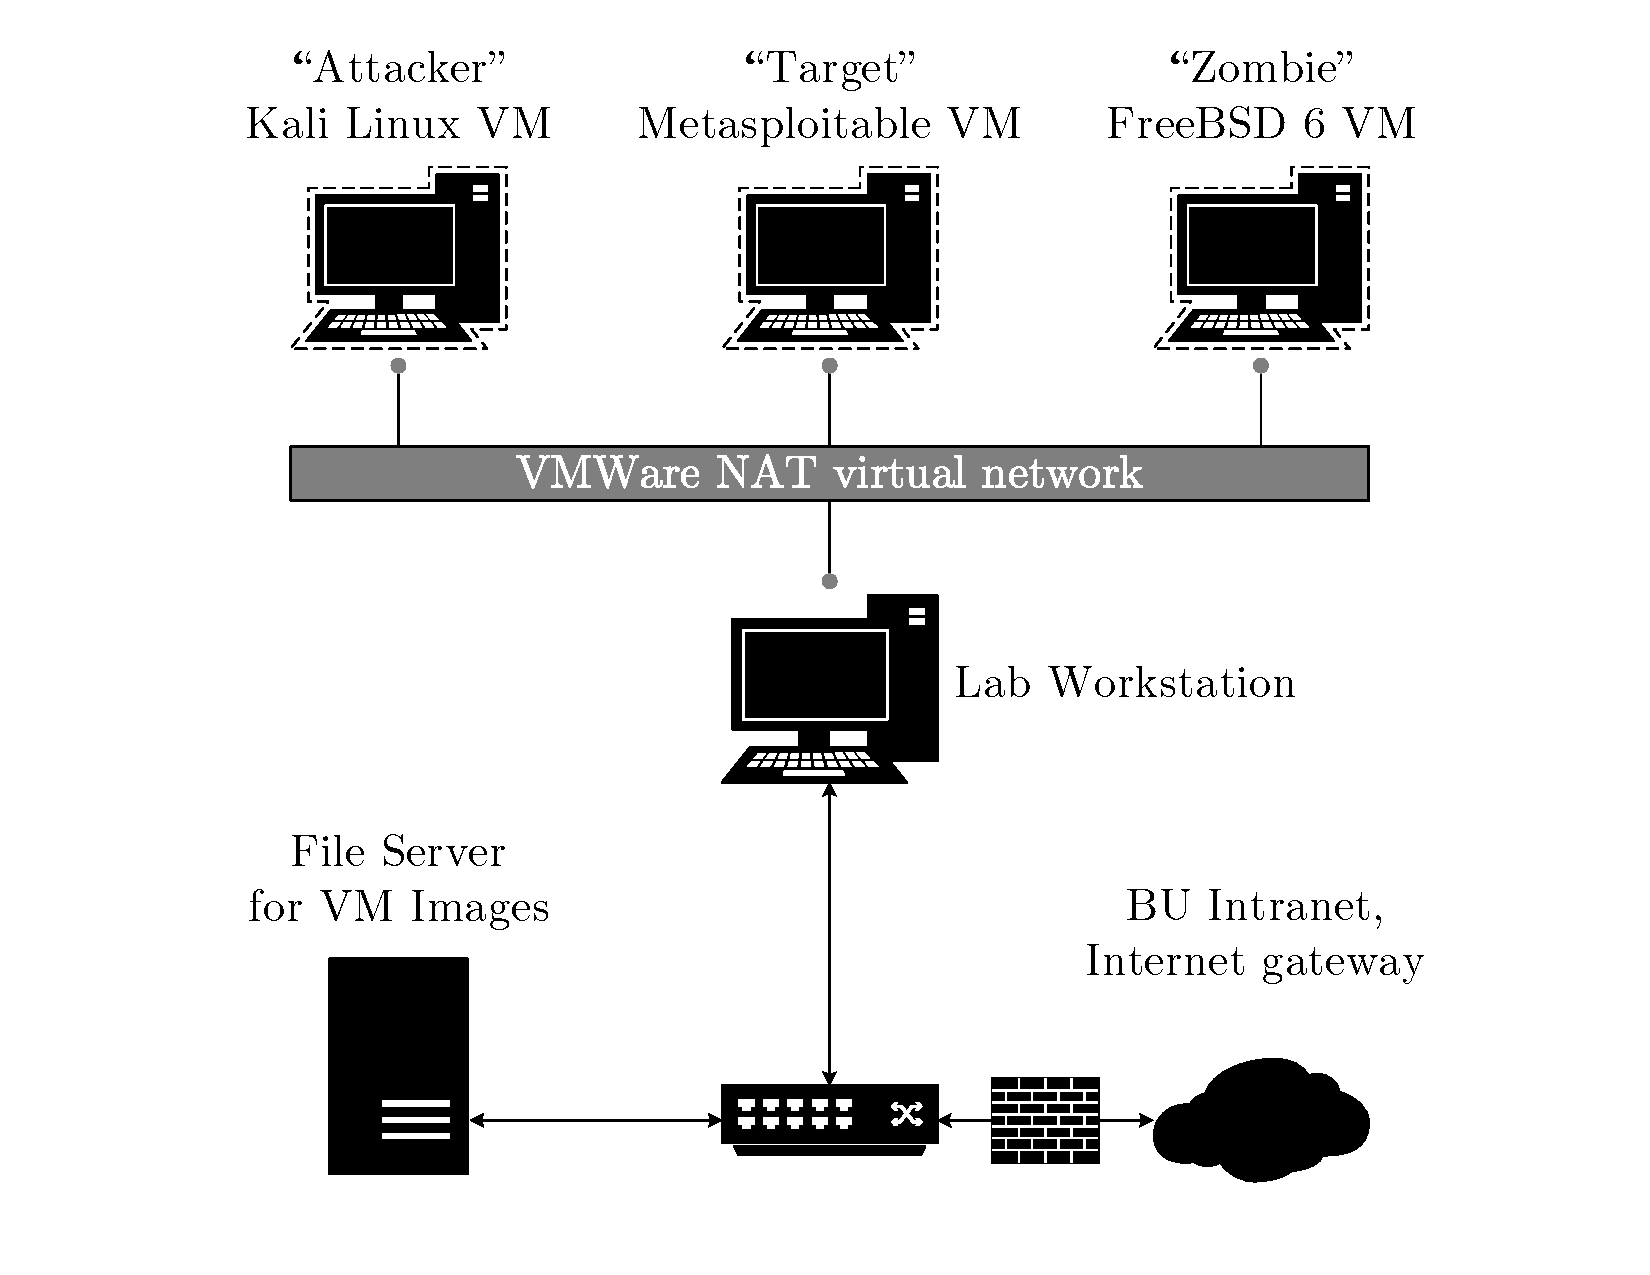
\includegraphics[scale=0.4, clip=true, trim=1.5in 0 0 0]{ec521_hostmap.pdf}
\caption{Diagram of the lab environment}
\label{fig:labenv}
\end{figure}

The networking laboratory is equipped with approximately 50 workstations with 4 Gb RAM running 
BU Linux \footnote{\url{http://www.bu.edu/tech/support/desktop/distribution/bulinux}}, 
a customized version of CentOS 6. Each machine runs VMWare Workstation 9.
Figure~\ref{fig:labenv} shows the connections for a single workstation, which has three virtual machines:

\begin{enumerate}
\item The attacker is represented by a \emph{Kali Linux} \cite{kali} virtual machine. This distribution is based
on Debian Linux, includes a multitude of security audit and penetration tools (including all the tools introduced
in the course), and is officially available for download as a VMWare image that boots into a desktop environment.
\emph{Kali} also includes a range of GUI tools that make some exploration possible even by users who may
not be comfortable with the underlying command line tools.
\item The target is represented by a \emph{Metasploitable 2} \cite{metavm} virtual machine. This image contains
a number of services with known exploits (ftp, http, and so on), insecure settings, and three vulnerable web 
applications. This VM is also officially available as a VMWare image, and has low memory requirements since it does
not offer a graphical user interface.
\item One of the assignments requires a third ``zombie'' machine. Almost any OS that has networking
support would do; we have chosen FreeBSD 6.0 for its low system requirements and for some diversity
in the virtual environment (i.e. not 100\% Linux). An unofficial VMWare image for this OS is publicly available \cite{tpolice}.
\end{enumerate}

Each student was provisioned a copy of the attacker and the target VM on a shared file server. The permissions
were set so that a student could access only their own copy of these VMs. These VMs were persistent--changes
made by students would be retained throughout the course.

A copy of both attacker and target VMs was also deployed locally on each workstation. These VMs were not 
persistent and would revert to their original contents whenever they were shut down. The purpose of these
VMs was to reduce the load on the network when working with the persistent image was not required, and to let
students experiment freely  without the risk of damaging their persistent VM. Students were instructed to use 
either their personal/persistent or the local/temporary VMs as they saw fit. 

For the lab requiring a ``zombie'' VM, the lab instructions provide a sequence of steps to download 
and run the additional VM on the workstation, offering a hands-on experience of obtaining and exploring a new OS.

The virtual network was configured to use network address translation (NAT), 
therefore all VMs could access the Internet but external access to VMs
was limited (no port forwarding was configured). This was done to let students practice installing additional packages
onto VMs and to allow Internet searches, etc. from the attacker VM itself.
An even more locked-down approach (that would also reduce the risk of students inadvertently launching an attack
on the lab network instead of the virtual LAN) would be to use the host-only networking mode.

\section{Lab Assignments}
A set of eight lab assignments has been developed for the course \cite{thelabs}. 
Each lab is accompanied by a comprehensive solution including relevant screenshots and further discussion.

\begin{figure}[b!]
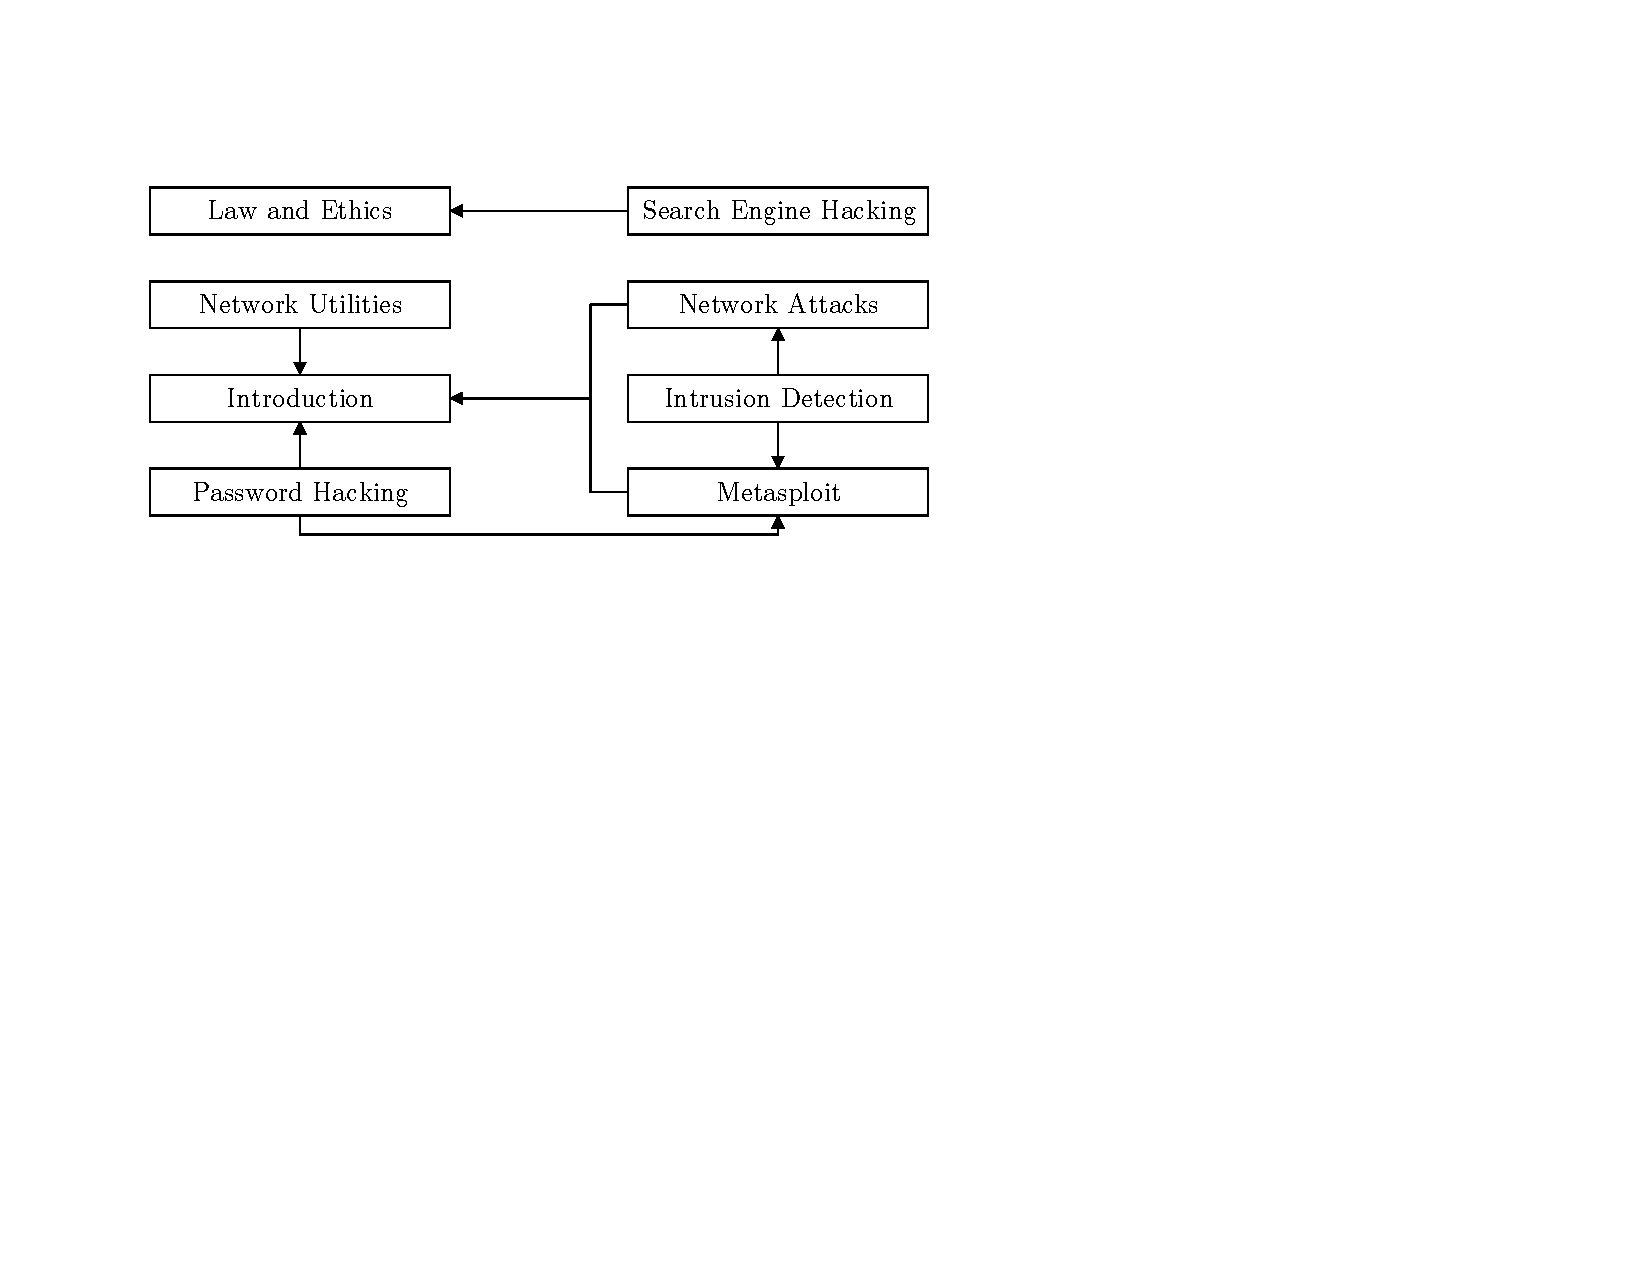
\includegraphics[scale=0.6, clip=true, trim=0.85in 5in 4.5in 1.2in]{dependencies-between-labs.pdf}
\caption{Dependencies between lab assignments}
\label{fig:labdeps}
\end{figure}

\begin{description}
\item[Law and Ethics] \hfill \\
This assignment is closer to a homework than a lab assignment, and asks students to evaluate various actions
in context of applicable law and ethics standards of relevant bodies (professional groups, Boston University, etc.)
\item[Introduction] \hfill \\
The first hands-on assignment introduces VMWare (the virtual environment) and the virtual machines used in the course
and guides a student through the installation and configuration process, as well as tests understanding of some
standard Linux tools and basic networking concepts.
\item[Search Engine Hacking and Social Engineering] \hfill \\
Students are asked to investigate an organization and discover relevant organizational and personal information
using a search engine, illustrating the amount of publicly available sensitive information that can routinely be found on the
Internet. Another part of the assignment poses several search questions that can be answered using search engine
queries with appropriate options, allowing search of historical website content (information that is no longer publicly
available but still present in Internet archives) and quick identification of instances of a vulnerable system.
\item[Network Utilities and Scripting] \hfill \\
Students explore various uses of common versatile network utilities (such as \texttt{netcat} and \texttt{wget}) and do some
scripting: in a shell script (utilizing the learned network utilities) and, on a lower level, by interacting with TCP/IP
sockets directly from the Python scripting language.
\item[Network Attacks] \hfill \\
This lab focuses on network attack tools included with Kali Linux. Specifically, ways to mount ARP and DNS
spoofing attacks on a network are demonstrated. The lab also asks students to do an \texttt{nmap} scan
uzing the ``zombie'' technique.
\item[Metasploit] \hfill \\ 
Using the \emph{Metasploit} framework, students are asked to perform several exploits on Metasploitable's
services that are known to be vulnerable, mount different denial-of-service attacks on a web server running
on the target VM, and explain why only some of the attacks are successful.
\item[Password Cracking] \hfill \\
The assignment introduces students to an off-line password cracking tool (\emph{John the Ripper}) and an on-line
tool (\emph{Hydra}) that can be used to guess passwords to a website requiring authentication. Students are asked to use the
on-line tool to find valid credentials to a different web application supplied with Metasploitable, and to crack 
Metasploitable's password database that they would download after compromising the target machine.
\item[Intrusion Detection] \hfill \\
A popular intrusion detection tool \texttt{snort} is introduced, students investigate varous modes of its operation
and develop a custom filter that detects a previously studied Metasploit exploit attempt on a specific service.
\end{description}

Whenever possible, the assignments reference topics that were covered by earlier labs. For example, the Network Attacks
lab walks students through using \texttt{ettercap} to perform ARP poisoning and tests their understanding of
the attack. A few weeks later, the Intrusion Detection lab asks students to ``perform ARP poisoning'' with the expectation
they already learned how to do it (or remember the previous lab and go to it for instructions). Figure~\ref{fig:labdeps} shows
the dependencies among the lab assignments.

\section{Discussion and Related Work}
We start the discussion with a brief overview of architectures for cybersecurity lab environments. 
For a longer survey, see Stewart et al \cite{virtplatform}.

Originally, cybersecurity labs started from mini-networks containing actual hardware. While offering
the most realism, such labs are expensive to acquire and maintain, and tend to fall behind state-of-the-art 
as new hardware is introduced. The choice of hardware limits the range of possible configurations and 
caps the number of students that can share a lab without interfering with each other.

The other option is a virtualized environment. Three classes of virtualized environments exist: 
\begin{itemize}
\item Centralized virtualization: a single server or a group of servers maintain virtual lab environments for all students, 
who access their environments remotely; one comprehensive centralized virtualization-based system is Tele-Lab \cite{willems2008tele}. 
\item Cloud virtualization: similar to centralized virtualization, substituting the underlying server resources with
data centers of the cloud services provider, and hosted hypervisors with the cloud provider's tools for spinning up, 
managing, and monitoring virtual server instances.  Salah \cite{salah2014harnessing} described an instance of this 
architecture on the Amazon Web Services platform.
\item Local virtualization (leveraging the resources of student workstations to maintain their virtual environments;
students have local access to their virtualized networks). This is the approach we have adopted.
\end{itemize}

Both centralized and cloud approaches carry some complexity and cost involved in setting up and maintaining the
environment. For organizations already having a server virtualization infrastructure, the former choice could be an attractive 
one; for organizations with limited on-site resources or technical personnel, the promise of ``infrastructure offloading''
to a cloud service may appear attractive but it comes with a bill for the resources consumed and does not really alleviate 
the demand for qualified technical staff to manage the environment.

The method of providing the entire virtual network on a single workstation benefits greatly from advances in
capabilities of modern hardware. For example, Stewart et al mentioned being able to run at most three virtual machines
using 256 MB each on a host with 1GB RAM in 2009 \cite{virtplatform}. At the time this lab was run, the three guest operating systems 
used 1.5 GB of RAM on a host equipped with 4 GB, using less than 50\% of the workstation's capacity. 

As RAM and core count of typical lab 
machines go up while the system requirements of virtualizing a small number of operating systems
and network devices remain roughly constant (since the relevant concepts can be demonstrated effectively on older
versions of operating systems), hosting such a selection of 10-20 devices (counting user machines and servers,
network hardware and filters/firewalls, and peripheral emulators) should be within capacity of a single modern  
workstation equipped with 16 GB RAM.

As a side effect of using commonly available software in a simple configuration, students could (and some of them did) 
use their personal laptops running Windows, Linux or OS X (with VMWare Fusion) to run the entire lab environment, 
including performing most of the lab assignments. There are several benefits to this flexibility: students can experiment
with the setup anywhere, not only at the lab; students are working with the host OS that is most familiar to them;
and it might well be that their personal laptop is more powerful and therefore runs the lab more smoothly than a lab
workstation. If this configuration is allowed, students should be instructed to use host-only networking mode: otherwise,
they could inadvertently use dangerous tools on any network they happen to be connected to.

Since we hosted persistent per-student virtual machine images on network storage, we were concerned 
with the possibility of ``long delays in copying large virtual machine images across the network for each student's work''  \cite{virtplatform}. 
We did not find this to be a problem in practice. This might be attributable to some students choosing to use 
local non-persistent VM images in the lab (or their own computers with local images), 
or to modern virtualization software being able to access only the data it needs
from a network hosted disk image, instead of copying the entire image to local storage.

\subsection{Scalability}

We would like to examine the scalability of each virtualization option (and of the set of labs) in the context of scaling up
to a large student audience, such as a MOOC (massive open online course) environment.

Out of the three virtualized approaches, centralized virtualization is the one most likely to run into scaling issues
as number of students grows and resource use approaches hardware capacity. Network use between virtual machines can
also become a bottleneck, particularly in scenarios that involve large amounts of traffic (DoS exercises, for example). It 
appears unlikely that most institutions would provision enough spare on-site capacity to deploy the environment 
for thousands of students.

Cloud virtualization enjoys a flexible and deep pool of resources, but the cost of maintaining the environment scales 
linearly with the number of students. Particularly in the context of the ``open'' (free) online course, the cost for the hosting
institution can escalate quickly. The complexity of managing a large number of students, particularly when not using any
dedicated tools beyond the standard cloud provider's provisioning user interfaces, can also explode in a non-linear fashion.
However, it would be possible to develop a specialized interface to handle specific user interface issues and enable both
a broad overview and a quick drill-down to a specific student's environment.

In contrast to the above approaches, scaling to a large number of local virtualized environments is fairly easy as each student
utilizes one standard computer (either university's or their own) to deploy the full environment. The remaining services (a
learning management system hosting the assignments, a file server hosting the VM images) are readily available at MOOC scales.
There are examples of MOOCs that have chosen this approach and have
run successfully with thousands of students.\footnote{For example, the \emph{Software Defined Networking} MOOC on Coursera
has provided a VirtualBox VM containing all the necessary tools for the course. \\ \url{https://class.coursera.org/sdn-002}.}

One potential issue with a locally hosted virtual environment is that the student's computer must be powerful enough to support it. This will 
inevitably not be the case for some students, who would have to seek alternative options. An interesting possibility could be
to deploy cloud instances only for those students, and have the students cover the costs of running those instances. 
\footnote{A relevant survey from the SDN MOOC: \\ \url{https://piazza.com/class/hvjn9udjegm75q?cid=426}}

\subsection{Didactic Materials}
\label{sec:labassignments}

There are several documented sets of lab assignments for cybersecurity courses. The set produced by the SEED project \cite{seed11} is 
perhaps the largest collection available that is designed specifically for instruction and 
uses a unified virtual environment (a version of Ubuntu) for most of the labs. It might be surprising, 
then, that there is not much overlap
between labs developed for this course and SEED labs; only the \emph{Network Attacks} lab corresponds to a SEED
\emph{TCP/IP Attack Lab}. Compared to SEED labs, which are often exploratory in nature, our labs offer more guidance
on the steps to perform and pose specific questions for students to answer, making them easier to grade and reducing
the overall time required to complete a lab.

Another set of labs is the \emph{OWASP Hackademic} \cite{hackademic}. Its original focus is web applications
security, and it uses a more involved setup to administer specific challenges. The authors do intend\footnote{``We intend to 
expand the available challenges with additional scenarios that involve cryptography, and even vulnerable systems 
implemented in download-able virtual machines.'' - \url{https://www.owasp.org/index.php/OWASP_Hackademic_Challenges_Project}
as of March 10, 2014} to expand the system to cover virtual machine-based security challenges, but at the time our
course was offered the functionality was not available.

There are many papers presenting one or more lab assignments that can be used in a cybersecurity course.
For example, Yuan et al \cite{yuan2014labsandtools} introduced two such labs: a wireless network attacks lab and a stack overflow lab.
However, with each such work offering only partial coverage of the course's intended topics, 
it would be a significant effort to reconcile labs from disparate sources
(having different setup requirements, writing style, level of difficulty and so on) into a harmonious set for the complete course.

It is worthwhile to note that our course plan includes an \emph{Laws and Ethics} lab early on, before any
tools and methods are introduced. Information security skills in general, and offensive security skills in particular, can
be used for both good and nefarious purposes, and covering the relevant laws, ethical principles, and guidelines at the outset
helps students evaluate their actions. While explicitly not technical, the importance of having an ethics lesson or lab early in
a course plan has been pointed out in previous work \cite{cook2012good}, 
but such a lesson is absent from both SEED and OWASP lab sets at this time. 

\subsection{Choice of Virtual Machines}

We have chosen to use \emph{Kali Linux} and \emph{Metasploitable} because these readily available images 
represent and teach the set of tools commonly used in the security industry and typical weaknesses that can be attacked using 
those tools respectively. Since both VMs were designed from the outset to be usable by individuals learning at their own pace 
and on their own equipment, the recommended environment already had to exclude anything that requires 
elaborate configuration or a complicated process.

Choosing a stable and popular environment that had all the necessary tools and required minimal modification enabled us 
to focus on creating content for the course instead of dealing with setting up a more elaborate system.

\subsection{Choice of Virtualization Software}

We used VMWare Workstation because the virtual machine images 
for both \emph{Kali Linux} and \emph{Metasploitable} 
were only ``officially'' available in VMWare format. VMWare Player can be
used for free by students to run the images on their computers, and a compatible 
Mac version (VMWare Fusion) exists. Furthermore, the university already had a 
license for VMWare software, so licensing cost was not a concern.

Image compatibility of virtualization software is constantly improving. We successfully
converted the VM images into VirtualBox \texttt{.ovf} format and verified several lab
questions to work. The instructions to do so, and the results of our testing in Parallels
on a Mac, will be posted to GitHub \cite{thelabs}.

\section{Student Feedback}

\begin{figure}[b!]
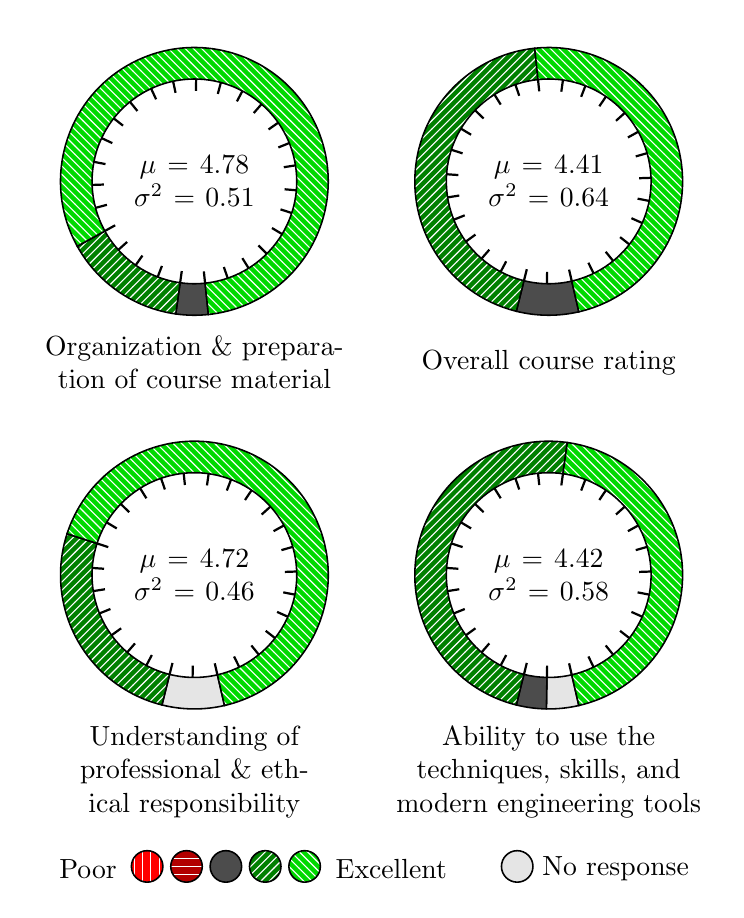
\begin{tikzpicture}
  \colorlet{scale1}{red}
  \colorlet{scale2}{red!70!black}
  \colorlet{scale3}{black!70}
  \colorlet{scale4}{green!50!black}
  \colorlet{scale5}{green!85!black}
  \colorlet{noresponse}{black!10}
  
  \node[align=center,text width=4cm] at (0cm, -2.3cm) {Organization \& preparation of course material};
  \node[align=center,text width=2.0cm] at (0,0) {$\mu=4.78$ \\ $\sigma^2=0.51$};

  \begin{scope}[rotate=-84]
    \newcount\mycount
    \foreach \angle in {0,13.333,...,359}
    {
      \mycount=\angle\relax
      \draw[black,thick] (\the\mycount:11.5mm) -- (\the\mycount:13.0mm);
    }  
	\draw[scale3] (0:1.5cm) arc (0:-14:1.5cm); 

	\filldraw[fill=scale3, line width=0.2mm] (0:1.7cm) arc (0:-14:1.7cm) -- (-14:1.3cm) arc (-14:0:1.3cm) -- cycle;

	\fill[fill=scale4, line width=0.2mm] (-14:1.7cm) arc (-14:-67:1.7cm) -- (-67:1.3cm) arc (-67:-14:1.3cm) -- cycle;	
	\filldraw[pattern=north east lines, pattern color=white, line width=0.2mm] (-14:1.7cm) arc (-14:-67:1.7cm) -- (-67:1.3cm) arc (-67:-14:1.3cm) -- cycle;	
	
	\fill[fill=scale5, line width=0.2mm] (-67:1.7cm) arc (-67:-360:1.7cm) -- (-360:1.3cm) arc (-360:-67:1.3cm) -- cycle;	
	\filldraw[pattern=north west lines, pattern color=white, line width=0.2mm] (-67:1.7cm) arc (-67:-360:1.7cm) -- (-360:1.3cm) arc (-360:-67:1.3cm) -- cycle;
  \end{scope}

    \node[align=center,text width=4cm] at (4.5cm, -2.3cm) {Overall course rating};
  \node[align=center,text width=2.0cm] at (4.5cm, 0cm) {$\mu = 4.41$ \\ $\sigma^2 = 0.64$};    
  \begin{scope}[xshift=4.5cm]    
  \begin{scope}[rotate=-77]
    \newcount\mycount
    \foreach \angle in {0,13.333,...,359}
    {
      \mycount=\angle\relax
      \draw[black,thick] (\the\mycount:11.5mm) -- (\the\mycount:13.0mm);
    }  
  
	\filldraw[fill=scale3, line width=0.2mm] (0:1.7cm) arc (0:-27:1.7cm) -- (-27:1.3cm) arc (-27:0:1.3cm) -- cycle;
	\fill[fill=scale4, line width=0.2mm] (-27:1.7cm) arc (-27:-187:1.7cm) -- (-187:1.3cm) arc (-187:-27:1.3cm) -- cycle;	
	\filldraw[pattern=north east lines, pattern color=white, line width=0.2mm] (-27:1.7cm) arc (-27:-187:1.7cm) -- (-187:1.3cm) arc (-187:-27:1.3cm) -- cycle;	
	\fill[fill=scale5, line width=0.2mm] (-187:1.7cm) arc (-187:-360:1.7cm) -- (-360:1.3cm) arc (-360:-187:1.3cm) -- cycle;	
	\filldraw[pattern=north west lines, pattern color=white, line width=0.2mm] (-187:1.7cm) arc (-187:-360:1.7cm) -- (-360:1.3cm) arc (-360:-187:1.3cm) -- cycle;
  \end{scope}  
  \end{scope}
  
  \node[align=center,text width=4cm] at (0cm, -7.5cm) {Understanding of professional \& ethical responsibility};
  \node[align=center,text width=2.0cm] at (0cm, -5cm) {$\mu = 4.72$ \\ $\sigma^2 = 0.46$};    
  \begin{scope}[yshift=-5cm]    
  \begin{scope}[line width=0.2mm,rotate=-77]
    \newcount\mycount
    \foreach \angle in {0,13.333,...,359}
    {
      \mycount=\angle\relax
      \draw[black,thick] (\the\mycount:11.5mm) -- (\the\mycount:13.0mm);
    }    
	\draw[fill=noresponse] (0:1.7cm) arc (0:-27:1.7cm) -- (-27:1.3cm) arc (-27:0:1.3cm) -- cycle;
	\fill[fill=scale4] (-27:1.7cm) arc (-27:-121:1.7cm) -- (-121:1.3cm) arc (-121:-27:1.3cm) -- cycle;	
	\filldraw[pattern=north east lines, pattern color=white] (-27:1.7cm) arc (-27:-121:1.7cm) -- (-121:1.3cm) arc (-121:-27:1.3cm) -- cycle;	
	\fill[fill=scale5, line width=0.2mm] (-121:1.7cm) arc (-121:-360:1.7cm) -- (-360:1.3cm) arc (-360:-121:1.3cm) -- cycle;	
	\filldraw[pattern=north west lines, pattern color=white, line width=0.2mm] (-121:1.7cm) arc (-121:-360:1.7cm) -- (-360:1.3cm) arc (-360:-121:1.3cm) -- cycle;	
  \end{scope}  
  \end{scope}  
  
  \node[align=center,text width=4cm] at (4.5cm, -7.5cm) {Ability to use the techniques, skills, and modern engineering tools};
  \node[align=center,text width=2.0cm] at (4.5cm, -5cm) {$\mu = 4.42$ \\ $\sigma^2 = 0.58$};    
  \begin{scope}[xshift=4.5cm, yshift=-5cm]    
  \begin{scope}[line width=0.2mm,rotate=-77]
    \newcount\mycount
    \foreach \angle in {0,13.333,...,359}
    {
      \mycount=\angle\relax
      \draw[black,thick] (\the\mycount:11.5mm) -- (\the\mycount:13.0mm);
    }    
  	\draw[fill=noresponse] (0:1.7cm) arc (0:-14:1.7cm) -- (-14:1.3cm) arc (-14:0:1.3cm) -- cycle;
  	\filldraw[fill=scale3] (-14:1.7cm) arc (-14:-27:1.7cm) -- (-27:1.3cm) arc (-27:-14:1.3cm) -- cycle;
	\fill[fill=scale4] (-27:1.7cm) arc (-27:-201:1.7cm) -- (-201:1.3cm) arc (-201:-27:1.3cm) -- cycle;	
	\filldraw[pattern=north east lines, pattern color=white] (-27:1.7cm) arc (-27:-201:1.7cm) -- (-201:1.3cm) arc (-201:-27:1.3cm) -- cycle;	
	\fill[fill=scale5, line width=0.2mm] (-201:1.7cm) arc (-201:-360:1.7cm) -- (-360:1.3cm) arc (-360:-201:1.3cm) -- cycle;	
	\filldraw[pattern=north west lines, pattern color=white, line width=0.2mm] (-201:1.7cm) arc (-201:-360:1.7cm) -- (-360:1.3cm) arc (-360:-201:1.3cm) 	 -- cycle;
  \end{scope}  
  \end{scope}
  
  \begin{scope}[xshift=-1.5cm, yshift=-8.7cm]
  \node at (0.15cm, -0.03cm) {Poor};
  \fill[scale1] (0.9, 0) circle (0.2cm);
  \filldraw[pattern=vertical lines, pattern color=white, line width=0.2mm] (0.9, 0) circle (0.2cm); 
  \fill[scale2] (1.4, 0) circle (0.2cm);
  \filldraw[pattern=horizontal lines, pattern color=white, line width=0.2mm] (1.4, 0) circle (0.2cm);
  \filldraw[fill=scale3, line width=0.2mm] (1.9, 0) circle (0.2cm);
  \fill[scale4] (2.4, 0) circle (0.2cm);
  \filldraw[pattern=north east lines, pattern color=white, line width=0.2mm] (2.4, 0) circle (0.2cm);
  \fill[scale5] (2.9, 0) circle (0.2cm);
  \filldraw[pattern=north west lines, pattern color=white, line width=0.2mm] (2.9, 0) circle (0.2cm);
  \node at (4cm, -0.03cm) {Excellent};  
  \filldraw[fill=noresponse, line width=0.2mm] (5.6cm, 0) circle (0.2cm);
  \node at (6.85cm, -0.03cm) {No response};
  \end{scope}
      
\end{tikzpicture}
\caption{Student survey results (27 respondents)}
\label{fig:survey}
\end{figure}

Towards the end of the semester, students were asked to fill an anonymous survey evaluating several teaching-related and
course-related questions. Each question uses a scale from 1 (poor) to 5 (excellent). Out of 38 students, 27 have
chosen to fill the survey; of those, 18\% identified as undergraduate and 67\% as graduate (15\% did not answer the question).
Figure~\ref{fig:survey} shows the responses to several of the questions asked on the survey.

The survey also allows students to write a freeform feedback about the course. The following are a few chosen responses:

\begin{quote}``The course was fun. I enjoyed the labs a lot. 
I~definitely learned quite a bit about cybersecurity from these labs alone.''\end{quote}

\begin{quote}``Strengths: in-class exercises and labs. Practical applications of the course tools helped to clarify
somewhat semantic [sic] lecture material\ldots''\end{quote}

\begin{quote}``Strong: good organization and explanation. Fun labs. Weak: even more hands-on would be great.''\end{quote}

A few students mentioned that the labs were too easy. Due to diverse background of students, we consciously chose
exercises and provided guidance such that our labs would be accessible to most students, accepting the fact 
that advanced students would find some of the labs too easy. A related survey question shows that a larger number 
of students do find the labs challenging and, on average, the difficulty is reasonable: 
14~students (52\% of respondents) rated the level of difficulty as ``average'', 
8~students (30\%) rated it ``too difficult'' and only one student rated the course ``easy''.

\section{Challenges and Future Work}

While Kali Linux (the attacker VM) has been updated every few months so far, the Metasploitable VM has been released in mid-2012
and saw no updates since. It remains usable as a snapshot, but if any changes have to be made to the image 
(for example, adding a package that was not installed by default) some workarounds and configuration changes
are already needed, as the base OS used for Metasploitable has transitioned from supported to archived status in 2013. As
such, and without explicit commitment to supporting Metasploitable going forward, its future and expansion are uncertain.

We have spent some effort modifying a Metasploitable image in an attempt to create a different environment for
the course's final exam (different available services, exploits, passwords and so on), but
adding new exploits was not possible due to limited time. The task would have been easier if the VM was designed in a modular,
customizable manner--for example, if it was possible to install vulnerable services from a pre-built package repository.

A single Linux VM is enough for a first cybersecurity course since it can demonstrate the relevant concepts. However,
the current computing environment is characterized by a multitude of popular architectures and operating systems.
A more realistic environment would include other vulnerable virtual machines based, for example, on Microsoft 
Windows XP and Mac OS X; and different architectures, for example Android on ARM providing an example
of a smartphone platform or Linux-based OpenWRT on MIPS32 for an example of a home router platform. 
We are not aware of an effort to provide such images specifically for cybersecurity training (with known security
holes and supporting didactic material), even as vulnerabilities in smartphone operating systems and embedded 
devices are making news throughout the tech industry.

Specifically for Windows XP, Metasploit exploits are available for the operating system itself (unpatched or on earlier service 
pack level), but obtaining known vulnerable (old) versions of third-party software has proven more difficult than authors
expected. Using a proprietary OS also carries licensing issues, but many institutions would have Windows XP licenses available
from previous deployments.

From the scalability perspective, the biggest challenge in scaling a cybersecurity course to a massively online audience is likely
to be in grading. MOOC classes typically use automated grading; developing a method to collect relevant output from different machines
of the local virtualized environment, automatically grading, and providing meaningful feedback for each of the proposed subject areas 
would be a big step forward towards enabling a MOOC instance of the course.

\section*{Acknowledgements}

The authors would like to acknowledge the contributions of James K. Goebel,
including the initial idea of switching to the virtual machine-based environment and technical aspects of the implementation,
which are not described in this paper since they are likely to be specific to Boston University's IT services % \balancecolumns \noindent 
configuration and therefore are of less general interest.

Yuguang Li and James Christianson wrote the initial versions of some of the
lab assignments mentioned in this paper and helped in testing the virtual course environment.

This research was supported in part by NSF under grants CNS-1012910 and CNS-1409053.

\printbibliography

\end{document}
